\chapter{Дифференцирование функций от одной переменной}

\section{Лекция \#16. Понятие дифференциала и дифференцируемости}

Мы теперь приступим к изучению функций которые локально действуют как растяжения или сжатия. Более формально это означает, что такие функции асимптотически приближаются линейными функциями.

\subsection{Понятие дифференциала}


\begin{definition}
Пусть $X,Y \subseteq \mathbb{R}$, функция $\varphi:X \to Y$ называется линейной если существует такое число $\alpha \in \mathbb{R}$, что
  \[
  \varphi(x) = \alpha \cdot x.
  \]
  для всех $x \in X.$
\end{definition}

\begin{mydanger}{\bf !}
  Интуитивно-геометрически это означает, что множество $X$ растягивается в $k$ раз, если $|k| >1$, или сжиматься в $k$ раз если $|k|<1$, и наконец отобразиться в точку $\{0\}$ если $k = 0.$
\end{mydanger}

К счастью, не все функции линейны, но некоторые очень похожи на них. Рассмотрим примеры.

\begin{example}
Рассмотрим функцию $f:\mathbb{R} \to \mathbb{R}$, $f(x) = x^2$ и некоторую точку $x_0\in \mathbb{R}$.

Имеем
 \begin{eqnarray*}
   f(x_0+h) &=& (x_0+h)^2 \\
    &=& x_0^2 + 2x_0h + h^2\\
    &=& f(x_0) + 2x_0\cdot h + h^2.
 \end{eqnarray*}

Это же равенство можно записать ещё так:
\[
 (x_0+h)^2 \approx x_0^2 + 2x_0\cdot h,
\]
при этом, чем меньше будет $h$, тем точнее будет результат. Например, если $h=0.1$, то получаем $1.1^2 =1.21$, а по нашей формуле $1.1^2 = (1+0.1)^2 \approx 1^2+ 2\cdot 1 \cdot 0.1 = 1.2$. С другой стороны, если $h=0.5$, то $1.5^2 = 2.25$, а по нашей формуле $1.5^2 = (1+0.5)^2 \approx 1^2 + 2\cdot 1 \cdot 0.5 = 1 + 1 = 2.$

Так как $h^2 = o(h)$, при $h\to 0$, то мы можем записать 
\[
 (x_0+h)^2 = x_0^2 + 2x_0\cdot h + o(h), \qquad h \to 0.
\]
\end{example}

Теперь мы готовы дать более формальное и строгое определение.

\begin{definition}\label{diff_of_function_on_R}
Пусть $\mathscr{U} \subseteq \mathbb{R}$ -- открытое подмножество. Говорят, что функция $f: \mathscr{U} \to \mathbb{R}$ \textit{дифференцируемо} в точке $x_0 \in \mathscr{U}$, если существует такое число $k_{x_0} \in \mathbb{R}$ (зависящее от точки $x_0$), что
\[
 f(x_0 + h)  = f(x_0) + k_{x_0}\cdot h + o(h), \qquad h\to 0.
\]

Если отображение дифференцируемо в каждой точке $\mathscr{U}$, то говорят, что она дифференцируема на $\mathscr{U}$.

Линейное отображение $\mathrm{d}f: \mathscr{U} \to \mathbb{R}$, $x_0 \mapsto k_{x_0}$ называется \textit{дифференциалом отображения} в точке $x_0 \in \mathscr{U}$. 
\end{definition}

\begin{example}
    Вернёмся ещё раз к функции $f:\mathbb{R} \to \mathbb{R}$, $x \mapsto x^2$. Так как
    \[
     (x_0 + h)^2 = x_0^2 + 2x_0\cdot h + h^2, 
    \]
\textit{т.е.,} $f(x_0 + h) = f(x_0) + 2x_0 \cdot h + o(h)$, при $h\to 0$, поэтому её дифференциал определяется так $(\mathrm{d}f)(x) = 2x$ для любого $x \in \mathbb{R}.$

Это значит, что локально, функция $f$ в конкретной точке $x_0$ делает растяжение с коэффициентом $2x_0$, \textit{т.е.,} $f$ ``очень похожа'' на линейную функцию, и эта линейная функция и называется дифференциалом $\mathrm{d}f$. В этом случае, она определяется так $\mathrm{d}f(x) = 2x$.
\end{example}

Прежде чем двигаться дальше, мы должны убедиться, что линейные отображения тоже дифференцируемы.

\begin{lemma}
 Любая линейная функция $\varphi: \mathscr{U} \to \mathbb{R}$ всюду дифференцируема на $\mathscr{U}$.
\end{lemma}
\begin{proof}
Действительно, так как $\varphi$ -- линейная функция, то существует такое число $k \in \mathbb{R}$, что $\varphi(x) = k\cdot x$. Тогда для любых $x,h \in \mathbb{R}$, имеем
\begin{eqnarray*}
 \varphi(x+h) &=& k\cdot (x+h) \\
 &=& k\cdot x + k \cdot h\\
 &=& \varphi(x) + \varphi(h).
\end{eqnarray*}

Таким образом, полагая теперь, что $(\mathrm{d}\varphi) (x)= k \cdot x$, и так как нулевая функция $0$, очевидно, лежит в $o(h)$, мы и получаем требуемое.
\end{proof}


Запись $f(x_0+h) = f(x_0)+k\cdot h + o(h),$ при $h \to 0$ означает также, что
\[
 k = \lim_{h \to 0} \frac{f(x_0 +h) - f(x_0)}{h}
\]
таким образом, дифференцируемость функции равносильна существованию этого предела.

\begin{definition}\label{derivative_of_function}
    \textit{Производная} функции $f(x)$ в точке $x_0$ -- это предел 
    \[
 \lim_{h\to 0} \frac{f(x_0 + h) - f(x_0)}{h},
    \]
    который принято обозначать одним из следующих образом: $f'(x_0)$, $\frac{d f}{dx}(x_0)$, а если -- $x$ это параметр времени, который обозначается обычно через $t$, то производную также обозначают как $\dot{f}(t_0)$.
\end{definition}

\begin{mydanger}{\bf{!}}
    Дифференциал -- это линейная часть приращения функции, а производная -- это предел отношения приращения функции к приращению аргумента при приращении аргумента, стремящемся к нулю. \textbf{Поэтому это не одно и тоже!!!}
\end{mydanger}


\begin{theorem}\label{diff=contionous_on_R}
    Если функция $f(x)$ дифференцируема в точке $x_0$, то она непрерывна в этой точке.
\end{theorem}

Нам нужно показать, что $\lim_{x \to x_0}f(x) = f(x_0)$, так как значение $f(x_0)$ по определению определено. Пусть $x:=x_0 +h$, тогда если $h \to 0$, то $x \to x_0$ и тогда из определения производной в точке $x_0$ следует, что существует предел
\[
 f'(x_0) = \lim_{x\to x_0} \frac{f(x) - f(x_0)}{x-x_0}.
\]

Имеем
\[
 f(x) - f(x_0) = \frac{f(x) - f(x_0)}{x-x_0}(x-x_0),
\]
тогда
\begin{eqnarray*}
     \lim_{x \to x_0} (f(x) - f(x_0))  &=& \lim_{x \to x_0}\frac{f(x) - f(x_0)}{x-x_0}(x-x_0) \\
     &=& f'(x_0) \lim_{x \to x_0}(x-x_0) \\
     &=& 0,
\end{eqnarray*}
\ie $\lim_{x \to x_0} f(x) = f(x_0)$, что и означает её непрерывность.\\

\begin{mydanger}{\bf{!}}
    В обратную сторону это неверно! То есть если функция непрерывна, то это вовсе не означает, что она дифференцируема.
\end{mydanger}

\subsection{Типичные не дифференцируемые функции}

Позже мы покажем, что если функция дифференцируема в точке, то к ней можно провести касательную в этой точке. Физически дифференцируемость функции от одной переменной означает, что скорость процесса (который описывается заданной функцией) меняется непрерывно от точки к точке, \ie не может быть мгновенного скачка скорости в какой-то точке.

\begin{example}\label{|x|is_not_diff}
    Рассмотрим функцию $f(x) = |x|$, покажем, что она не дифференцируема точке $x_0 =0$.

\begin{figure}
    \centering
    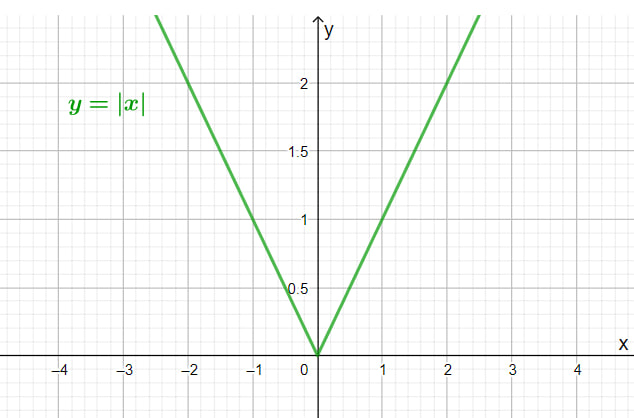
\includegraphics{images/abs(x).jpg}
    \caption{График функции $f(x) = |x|.$}
    \label{fig:enter-label}
\end{figure}
    
    Рассмотрим предел
    \begin{eqnarray*}
        \lim_{x \to 0}\frac{f(x) - f(0)}{x - 0} &=& \lim_{x \to 0} \frac{|x| - 0}{x-0} \\
        &=&\lim_{x \to 0} \frac{|x|}{x}\\
        &=& \lim_{x \to 0}\mathrm{sign}(x),
    \end{eqnarray*}
    где $\mathrm{sign}(x) : = \begin{cases}
        1, & x > 0, \\
        0, & x =0, \\
        -1 , & x <0,
    \end{cases}$
    но эта функция не непрерывна в точке $x_0$, а значит, и нет предела $\lim_{x \to 0}\frac{f(x) - f(0)}{x - 0}$, что и означает, что эта функция недифференцируема в точке $x_0 = 0.$

\end{example}

\begin{figure}[h!]
    \centering
    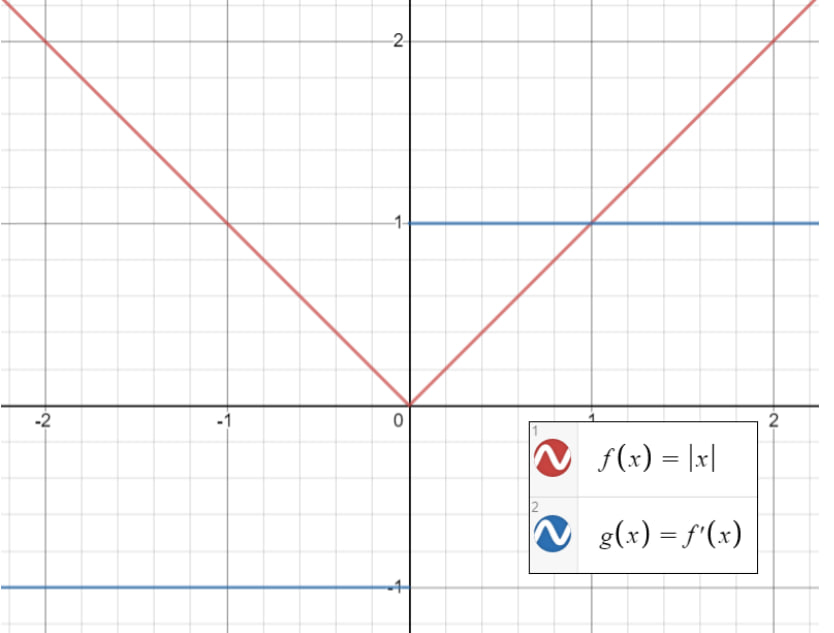
\includegraphics[scale = 0.7]{images/abs(x)+sign(x).jpg}
     \caption{Красным показан график функции $f(x) = |x|$, а синим -- график функции $g(x) = \mathrm{sign}(x)$, мы видим, что $g(x)$ делает резкий скачок в точке $0$, что и означает, что функция $f(x)$ недифференцируема.}
\end{figure}


\begin{example}
Одним из самых ярких контрпримеров является функция Вейерштрасса -- всюду непрерывная, но нигде не дифференцируемая функция. 
Аналитически она записывается следующим образом:

\[
f(x) = \sum_{n=0}^{\infty} {a^n \cos(b^n \pi x)},
\]
где $0 < a < 1, \; b$ -- положительное нечётное целое и
\[
ab > 1 + \frac{3 \pi}{2}
\]


\begin{figure}[h!]
    \centering
    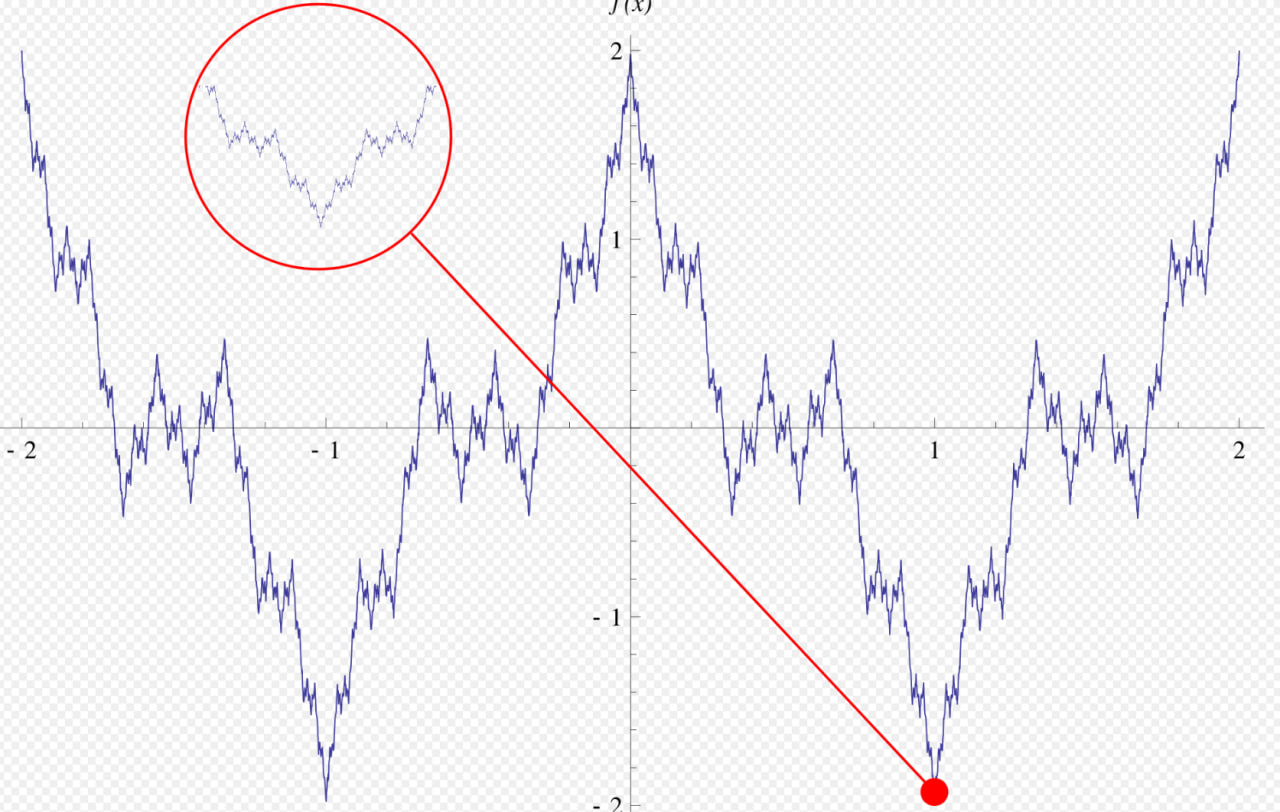
\includegraphics[width=1\linewidth]{images/WeierstrassFunction.jpeg}
    \caption{Простыми словами, функция Вейерштрасса резко меняет своё направление в каждой точке, поэтому не может быть дифференцируемой, но она также всюду непрерывна как предел равномерно сходящихся всюду непрерывных частичных сумм.    }
\end{figure}
\end{example}

\subsection{Свойства производной}

\begin{theorem}\label{ariph_for_der}
    Если функции $f(x), g(x)$ дифференцируемы в точке $x_0$, то:
    \begin{enumerate}
        \item $(f+g)'(x_0) = f'(x_0) + g'(x_0)$;
        \item $(fg)'(x_0) = f'(x_0) g(x_0) + f(x_0) g'(x_0);$
        \item $\left( \dfrac{f}{g} \right)'(x_0) = \dfrac{f'(x_0)g(x_0) - f(x_0) g'(x_0)}{(g(x_0))^2}$
    \end{enumerate}
\end{theorem}
\begin{proof}~

(1) Это сразу следует из того, что предел суммы -- это сумма пределов.

(2) Имеем
\begin{eqnarray*}
    (fg)'(x_0) &:=& \lim_{x \to \to x_0} \frac{f(x)g(x) - f(x_0)g(x_0)}{x-x_0} \\
    &=& \lim_{x \to x_0} \frac{ f(x)g(x)  - f(x_0) g(x) + f(x_0) g(x) - f(x_0)g(x_0)  }{x-x_0} \\
    &=& \lim_{x \to  x_0} \frac{ (f(x) - f(x_0))g(x)  + f(x_0) ( g(x) - g(x_0) )  }{x-x_0},
\end{eqnarray*}

По условию $f,g$ -- дифференцируемы в точке $x_0$, тогда согласно теореме \ref{diff_of_function_on_R}, $f,g$ -- непрерывны в точке $x_0$, а тогда согласно теореме \ref{criteria_of_continous} $\lim_{x\to x_0} f(x) = f(x_0)$ и $\lim_{x\to x_0}g(x) = g(x_0)$. 

Используя теперь арифметику предела (см. Теорему \ref{lim(f+g)}), получаем
\begin{eqnarray*}
    (fg)'(x_0) &=& \lim_{x \to  x_0} \frac{ (f(x) - f(x_0))g(x)  + f(x_0) ( g(x) - g(x_0) )  }{x-x_0} \\
    &=& \lim_{x \to x_0} \frac{f(x) - f(x_0)}{x-x_0} \cdot \lim_{x \to x_0} g(x) + f(x_0) \cdot \lim_{x \to x_0} \frac{g(x) - g(x_0)}{x-x_0} \\
    &=& f'(x_0)\cdot g(x_0) + f(x_0)\cdot g'(x_0).
\end{eqnarray*}

(3) Имеем
\begin{eqnarray*}
    \left( \dfrac{f}{g} \right)'(x_0) &=& \lim_{x\to x_0} \dfrac{ \dfrac{f(x)}{g(x)} - \dfrac{f(x_0)}{g(x_0)} }{x-x_0} \\
    &=& \lim_{x\to x_0} \left( \frac{f(x) g(x_0) - f(x_0) g(x)}{x-x_0}\cdot \frac{1}{g(x) g(x_0)} \right)\\
    &=& \lim_{x \to x_0}\left( \dfrac{f(x) g(x_0) - f(x_0)g(x_0) + f(x_0)g(x_0) - f(x_0)g(x)}{x-x_0} \cdot \frac{1}{g(x) g(x_0)} \right).
\end{eqnarray*}

Опять по условию $f,g$ -- дифференцируемы в точке $x_0$, тогда согласно теореме \ref{diff_of_function_on_R}, $f,g$ -- непрерывны в точке $x_0$, а тогда согласно теореме \ref{criteria_of_continous} $\lim_{x\to x_0} f(x) = f(x_0)$ и $\lim_{x\to x_0}g(x) = g(x_0)$. 

Используя теперь арифметику предела (см. Теорему \ref{lim(f+g)}), получаем
\begin{eqnarray*}
   \left( \dfrac{f}{g} \right)'(x_0) &=& \lim_{x \to x_0}\left( \dfrac{f(x) g(x_0) - f(x_0)g(x_0) + f(x_0)g(x_0) - f(x_0)g(x)}{x-x_0} \cdot \frac{1}{g(x) g(x_0)} \right) \\
   &=& \lim_{x \to x_0}\left( \dfrac{f(x) g(x_0) - f(x_0)g(x_0) + f(x_0)g(x_0) - f(x_0)g(x)}{x-x_0}\right) \cdot\left( \lim_{x\to x_0} \frac{1}{g(x) g(x_0)} \right) \\
   &=& \frac{1}{(g(x_0))^2}\cdot \cdot \left( \lim_{x \to x_0} \frac{f(x) - f(x_0)}{x-x_0}\cdot g(x_0)  - f(x_0) \cdot \lim_{x\to x_0} \frac{g(x) - g(x_0)}{x-x_0}  \right) \\
   &=& \frac{f'(x_0)g(x_0) - f(x_0)g'(x_0)}{(g(x_0))^2}.
\end{eqnarray*}



\end{proof}






\begin{theorem}\label{d(fg)}
Пусть $f: \mathscr{U} \to \mathbb{R}$ дифференцируема в $x_0 \in \mathscr{U}$, $g: \mathscr{W} \to \mathbb{R}$ дифференцируема в $y_0= f(x_0)$. Тогда $g \circ f :\mathscr{U} \to \mathbb{R}$ дифференцируемa в $x_0$ и 
    \[
   \mathrm{d} ( g\circ f)_{x_0} = (\mathrm{d}g)_{y_0} \cdot (\mathrm{d}f)_{x_0}.
    \]
\end{theorem}


\begin{proof}

 Так как $f$ дифференцируема, мы имеем
 \[
 f(x_0 + h) - f(x_0) = (\mathrm{d}f)_{x_0}(h) + \alpha(h) \cdot h,
 \] 
 и
 \[
  g(f(x_0) + v)) - g(f(x_0)) = (\mathrm{d}g)_{y_0}(v) + \beta(v)\cdot v
 \]
где $\lim_{h \to 0} \alpha (h) = 0$, $\lim_{v \to 0} \beta (v) = 0$.

Тогда, согласно определению предела (см. Определение \ref{the_main_def_of_limit_on_R}), мы можем положить $\alpha(0), \beta(0) := 0$.

Пусть $v: =f(x_0 + h) - f(x_0)$. Так как, согласно условию $f$ -- дифференцируема в точке $x_0$, тогда (см. Теорема \ref{diff_of_function_on_R}) она непрерывна в точке $x_0$, а тогда (см. Теорему \ref{criteria_of_continous}), если $h\to 0$, то $v \to 0$. 

Имеем

\begin{eqnarray*}
    g(f(x_0 +h)) -g(f(x_0)) &=& (\mathrm{d}g)_{y_0} \cdot \bigl(f(x_0+h) - f(x_0)\bigr)  \\
    &+& \beta\Bigl( f(x_0+h) - f(x_0) \Bigr) \cdot (f(x_0+h) - f(x_0)) \\
    &=& (\mathrm{d}g)_{y_0} \Bigl( (\mathrm{d}f)_{x_0}(h) + \alpha(h) \cdot h\Bigr) \\
    &+& \beta\Bigl(  (\mathrm{d}f)_{x_0}(h) + \alpha(h) \cdot h \Bigr) \cdot \Bigl(  (\mathrm{d}f)_{x_0}(h) + \alpha(h) \cdot h \Bigr)
\end{eqnarray*}
из-за линейности $(\mathrm{d}g)_{y_0}$ получаем
\begin{eqnarray*}
    g(f(x_0 +h )) -g(f(x_0)) &=&\Bigl((\mathrm{d}g)_{y_0 } \cdot (\mathrm{d}f)_{x_0}\Bigr) (h) + (\mathrm{d}g)_{ y_0} \cdot \alpha( h) \cdot h \\
    &+& \beta\Bigl( (\mathrm{d}f)_{x_0}\cdot h + \alpha(h) \cdot h \Bigr) \cdot \Bigl(  (\mathrm{d}f)_{x_0}\cdot h + \alpha(h) \cdot h \Bigr).     
\end{eqnarray*}

Запишем теперь это равенство так

\begin{eqnarray*}
    g(f(x_0 +h )) -g(f(x_0)) &=&\Bigl((\mathrm{d}g)_{y_0 } \cdot (\mathrm{d}f)_{x_0}\Bigr) (h) + (\mathrm{d}g)_{ y_0} \cdot \alpha( h) \cdot h \\
    &+& \beta\Bigl( \bigl( (\mathrm{d}f)_{x_0}+ \alpha(h) \bigr) \cdot h \Bigr) \cdot \Bigl(  (\mathrm{d}f)_{x_0} + \alpha(h) \Bigr)\cdot h.     
\end{eqnarray*}

Положим
\[
 \gamma(h): = (\mathrm{d}g)_{ y_0} \cdot \alpha( h)  + \beta\Bigl( \bigl( (\mathrm{d}f)_{x_0}+ \alpha(h) \bigr) \cdot h \Bigr) \cdot \Bigl(  (\mathrm{d}f)_{x_0} + \alpha(h) \Bigr),
\]
тогда
\[
  g(f(x_0 +h )) -g(f(x_0)) = \Bigl((\mathrm{d}g)_{y_0 } \cdot (\mathrm{d}f)_{x_0}\Bigr) (h) + \gamma(h)\cdot h.
\]

В силу непрерывности $\alpha(h), \beta(h)$ в точке $h=0$ и существования в точке $x_0$ дифференциалов $(\mathrm{d}f)_{x_0}:=f'(x_0)$, $(\mathrm{d}g)_{y_0}:=g'(y_0)$, мы, используя теорему о композиции (см. Теорема \ref{comp_of_continous_on_R}), тогда получаем
\begin{eqnarray*}
 \lim_{h \to 0} \gamma(h) &=& \lim_{h\to 0} \Bigl( (\mathrm{d}g)_{ y_0} \cdot \alpha( h)  + \beta\Bigl( \bigl( (\mathrm{d}f)_{x_0}+ \alpha(h) \bigr) \cdot h \Bigr) \cdot \Bigl(  (\mathrm{d}f)_{x_0} + \alpha(h) \Bigr) \Bigr) \\
 &=& (\mathrm{d}g)_{ y_0} \cdot \lim_{h\to 0} \alpha( h)  + \beta\Bigl( \bigl( (\mathrm{d}f)_{x_0}+  \lim_{h\to 0}\alpha(h) \bigr) \cdot \lim_{h\to 0} h \Bigr) \cdot \Bigl(  (\mathrm{d}f)_{x_0} + \lim_{h\to 0}\alpha(h) \Bigr) \\
 &=& 0 + \beta(0)\cdot (f'(x_0))\\
 &=& 0.
\end{eqnarray*}

Тогда мы показали, что
\[
 g(f(x_0 +h )) -g(f(x_0)) =\Bigl((\mathrm{d}g)_{y_0 } \cdot (\mathrm{d}f)_{x_0}\Bigr) (h) + o(h), \qquad h \to 0 
\]
или
\[
 g(f(x_0 +h ))  = g(f(x_0))+\Bigl((\mathrm{d}g)_{y_0 } \cdot (\mathrm{d}f)_{x_0}\Bigr) (h) + o(h), \qquad h \to 0
\]
откуда
\[
\mathrm{d}(g\circ f)_{x_0} = (\mathrm{d}g)_{y_0 } \cdot (\mathrm{d}f)_{x_0},
\]
что и доказывает утверждение.
\end{proof}



\subsection{Геометрический смысл дифференциала функции}



\begin{theorem}
    Пусть функция $f(x)$ дифференцируема в точке $x_1$, а прямая $\ell$, проходящая через точки $(x_1,y_1)$, $(x_2,y_2)$, где $y_1 = f(x_1)$, $y_2 = f(x_2)$, задаётся уравнением $y = k(x_2) (x - x_1 ) + y_1$. Тогда
    \[
     \lim_{x_2 \to x_1} k(x_2) = f'(x_1).
    \]
\end{theorem}
  
\begin{figure}[h!]
    \centering
    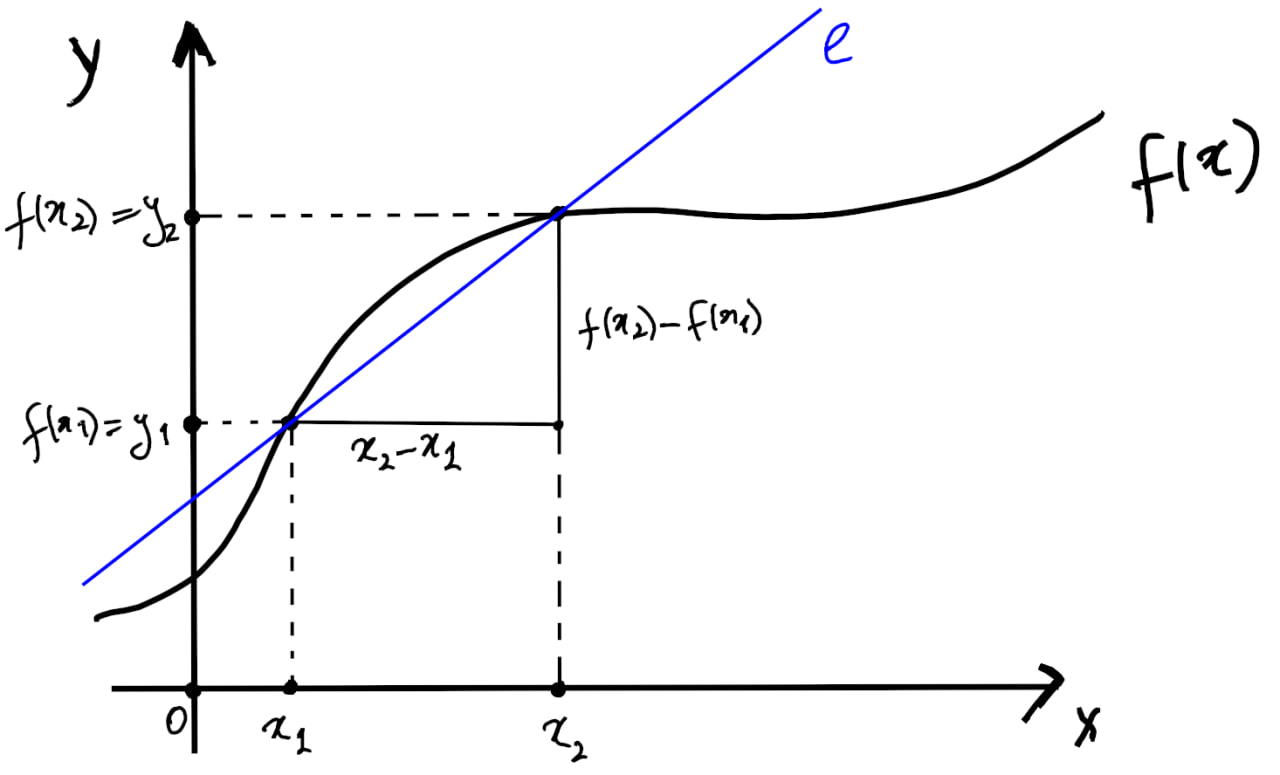
\includegraphics[scale = 0.4]{images/line_and_f'.jpg}
    \caption{Прямая $\ell$, проходящая через точки $(x_1,y_1)$, $(x_2,y_2)$, где $y_1 = f(x_1)$, $y_2 = f(x_2)$}
    \label{fig:enter-label}
\end{figure}

\begin{proof}
    Рассматриваемая прямая задаётся уравнением 
\[
 y = \frac{f(x_2) - f(x_1)}{x_2 - x_1}(x-x_1) +y_1,
\]
поэтому
\[
 k(x_2)  = \frac{f(x_2) - f(x_1)}{x_2 - x_1}.
\]

Тогда из определения производной следует, что
\[
 \lim_{x_2 \to x_1}k(x_2) = f'(x_1).
\]
\end{proof}

\begin{definition}
    Прямую $y = f'(x_0)(x-x_0) + f(x_0)$ называют \textit{касательной} к графику $y = f(x)$ в точке $(x_0, f(x_0)).$
\end{definition}

\begin{figure}[h!]
    \centering
    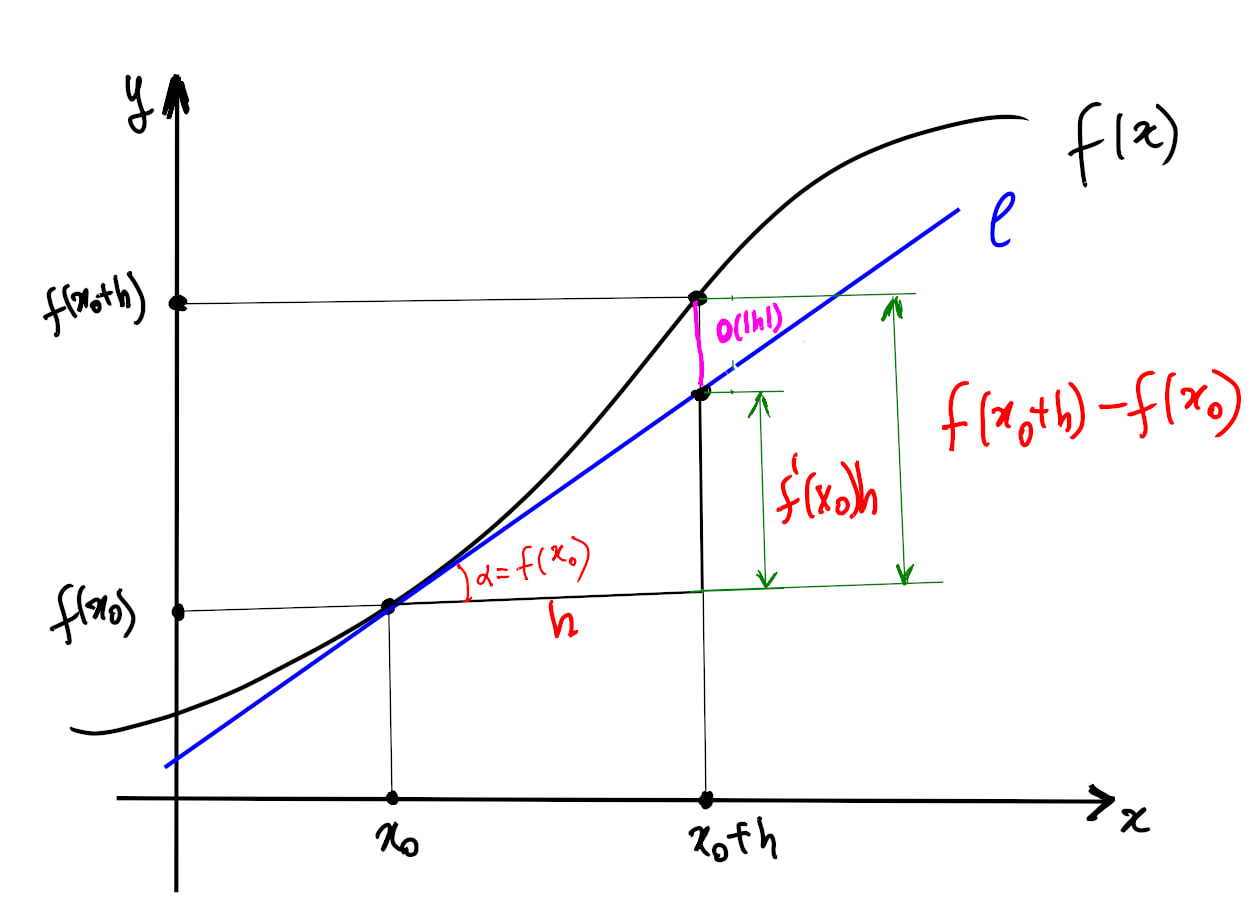
\includegraphics[scale= 0.4]{images/tan_and_f.jpg}
    \caption{Таким образом, если функция $f(x)$ дифференцируема в точке $x_0$, то её можно приблизить линейной функцией $f'(x_0)(x-x_0) +f(x_0)$, при этом $o(h)$ показывает, насколько далеко это приближение.}
    \label{fig:enter-label}
\end{figure}





\section{Лекция \#17. Функции на компактном множестве}

Как мы знаем (см. Теорема \ref{criterai_of_compacness_in_R}), любое компактное множество на $\mathbb{R}$ содержится в отрезке, то все наши рассуждения будут вестись над отрезком конечной длины.

\subsection{Непрерывность на компактном множестве}

\begin{theorem}[о промежуточном значении]\label{intermediat_theorem}
 Если функция $f(x)$ непрерывна на отрезке $[a,b]$ и принимает на его концах значения разных знаков, то $f(x_0) = 0$ для некоторой точки $x_0 \in [a,b]$.    
\end{theorem}
\begin{proof}
    Пусть $f(a)>0$, $f(b)<0$.  Построим последовательности $(a_n)$, $(b_n)$ следующим образом; $a_1:=a$, $b_1:=b$,
\begin{align*}
    &a_{n+1}:= \begin{cases}
        \frac{a_n +b_n}{2}, & \mbox{если $f(\frac{a_n +b_n}{2})>0$},\\
        a_n, & \mbox{если $f(\frac{a_n +b_n}{2})<0$},
    \end{cases}  & b_{n+1}:= \begin{cases}
        \frac{a_n +b_n}{2}, & \mbox{если $f(\frac{a_n +b_n}{2})<0$},\\
        b_n, & \mbox{если $f(\frac{a_n +b_n}{2})>0$},
        \end{cases}
\end{align*}
при $n\ge 1$.

Покажем, что $a_{n+1}\le b_{n+1}$. По условию $a_1: = a < b =:b_1$. Пусть $a_n \le b_n$. Рассмотрим тогда $a_{n+1}$, $b_{n+1}$. Тогда, если $a_{n+1} = \frac{a_{n}+b_n}{2}$. то $b_{n+1} = b_n$, и тогда 
\[
 a_{n+1} = \frac{a_n+b_n}{2} < \frac{b_n + b_n}{2} = b_n = b_{n+1}.
\]
Если же $a_{n+1} = a_n$, то $b_{n+1} = \frac{a_n + b_n}{2}$, и мы получаем
\[
 b_{n+1} = \frac{a_n + b_n}{2} > \frac{a_n + a_n}{2} = a_n = a_{n+1}.
\]

Итак, мы показали, что $a_n \le b_n$. Далее покажем, что $a_{n+1} \ge a_n$. Действительно, либо $a_2= a_1$, либо $a_2 = \frac{a_1 + b_1}{2} = \frac{a+b}{2} > \frac{a+a}{2} = a = a_1$. Пусть $a_{n} \ge a_{n-1}$, тогда если $a_{n+1} = \frac{a_n + b_n}{2}$, то $b_{n+1} = b_n$, то
\[
 a_{n+1} = \frac{a_n + b_n}{2} \ge \frac{a_n + a_n}{2} = a_n,
\]
иначе $a_{n+1} = a_n$.

Аналогично показывается, что $b_{n+1} \le b_{n}$.

В итоге, мы получили две ограниченные\footnote{потому что они находятся в отрезке!} монотонные последовательности $(a_n)$, $(b_n)$. Тогда по теореме Вейерштрасса \ref{Weierstrass} у них есть предел.

С другой стороны, имеем
\[
 b_{n+1} - a_{n+1} = \begin{cases}
      \frac{a_n+b_n}{2} - a_n = \frac{b_n - a_n}{2}, & \mbox{если $b_{n+1} = \frac{a_n + b_n}{2}$ и тогда $a_{n+1} = a_n$}, \\
      b_n - \frac{a_n + b_n}{2} = \frac{b_n - a_n}{2}, & \mbox{если $b_{n+1} = b_n$ и тогда $a_{n+1} = \frac{a_n + b_n}{2}$}
 \end{cases}, 
\]
\ie
\[
 b_{n+1} - a_{n+1} = \frac{b_n - a_n}{2} =  \frac{b - a}{2^{n}}.
\]
\end{proof}

Тогда получаем
\[
 \lim_{n \to \infty} (b_n - a_n) = \lim_{n \to \infty} \frac{b-a}{2^{n-1}} =0,
\]
\ie $\lim_{n \to \infty} a_n = \lim_{n \to \infty} b_n =x_0.$

Так как функция непрерывна, и $x_0$ есть точка прикосновения отрезка $[a,b]$, то по теореме  \ref{lim=>for_any_sequence}, $f(x_0) = \lim_{n \to \infty} f(a_n) = \lim_{n \to \infty} f(b_n)$. С другой стороны, по построению последовательности все $f(a_n) \ge 0$, $f(b_n)\le 0$, тогда по теореме \ref{lim(f+g)},
\[
 \lim_{n \to \infty} f(a_n)\ge 0, \qquad  \lim_{n \to \infty} f(b_n)\le 0,
\]
 но тогда $f(x_0) =  \lim_{n \to \infty} f(a_n) =  \lim_{n \to \infty} f(b_n) = 0$, что и требовалось. 


\begin{mydangerr}{\bf!}
 Эту теорему формулируют также следующим образом.
\end{mydangerr}

\begin{corollary}\label{mean_value_theorem}
    Пусть функция $f:[a,b] \to \mathbb{R}$ -- непрерывная функция, пусть $f(a) \ne f(b)$, и без ограничения общности предположим, что $f(a) < f(b)$, тогда для любого $\xi\in [f(a), f(b)]$ существует такой $x_0 \in [a,b]$, что $f(x_0) = \xi.$
\end{corollary}

\begin{proof}
    Действительно, для лююбого фиксированного числа $f(a) \le \xi \le f(b)$, функция $g_\xi(x) := f(x) - \xi$ является непрерывной на $[a,b]$ ибо она есть сумма непрерывных функций. Далее, $g(a) = f(a) - \xi <0$ и $g(b) = f(b) - \xi >0$, тогда согласно предыдущей теореме, найдётся такой $x_0 \in [a,b]$, что $f(x_0) = \xi$, что и требовалось доказать.
\end{proof}

\begin{definition}
    Значение функции, которое является наибольшим или наименьшим, называется \textit{экстремальным}. Точку, в которой функция принимает экстремальное значение, называют \textit{точкой экстремума}. Если же рассматривается какая-то окрестность точки $x_0$ и оказывается, что $x_0$ точка экстремума, то говорят, что $x_0$ есть точка \textit{локального экстремума.} 
\end{definition}


\begin{theorem}\label{continous_on_interval_on_R}
    Функция $f(x)$, непрерывная на отрезке $[a,b]$, ограничена на этом отрезке.
\end{theorem}
\begin{proof}
    Докажем, что она ограничена сверху (ограниченность снизу доказывается аналогично). Пусть для любого $n\in \mathbb{N}$ на отрезке $[a,b]$ есть такая точка $x_n$, что $f(x_n) >n$. Мы получаем ограниченную последовательность $(x_n)$, тогда по теореме \ref{from_bounded_sequence} можно выбрать сходящуюся подпоследовательность $(x_{n_k})$. Пусть тогда $\lim_{n\to \infty}x_{n_k} = x_0$. Согласно лемме \ref{a<b}, $a\le x_0 \le b$. 

    Далее, так как $f(x)$ непрерывна на всём отрезке, то $f(x_0) = \lim_{x\to x_0}f(x)$, но тогда, согласно теореме \ref{lim=>for_any_sequence}, $f(x_0)  = \lim_{n\to \infty} f(x_{n_k})$, но мы предположили, что $f(x_{n_k}) > n_k$, тогда $\lim_{n\to \infty} f(x_{n_k}) = \infty$, что даёт противоречие.
\end{proof}

\begin{theorem}(Вейерштрасс)\label{W2_on_R}
    Функция $f(x)$, непрерывная на отрезке $[a,b]$, достигает максимума и минимума в некоторых точках этого отрезка.
\end{theorem}
\begin{proof}

Рассмотрим множество $\Bigl\{f(x),\, x \in [a,b] \Bigr\}$. Очевидно, что оно не пусто. Согласно теореме \ref{continous_on_interval_on_R}, оно ограничено. Тогда, согласно принципу полноты Вейерштрасса (теорема \ref{W=complete}), это множество имеет $\sup$ и $\inf$.

Покажем\footnote{для $\inf$ доказательство аналогичное}, что на отрезке $[a,b]$ есть такая точка $x_0$, для которой $f(x_0) = M$, где
\[
M: = \sup_{a \le x \le b}\{f(x)\}.
\]

Итак, множество $\Bigl\{f(x),\, x\in  [a,b] \Bigr\}$ ограничено и не пусто и имеет $\sup, \inf$. Тогда из определения \ref{sup,inf} следует, что найдутся такие $f(x_n)$, что 
$$M - \frac{1}{n} \le f(x_n) \le M$$
для какой-то последовательности $(x_n)$ точек из $[a,b]$. Согласно теореме \ref{from_bounded_sequence}, можно выбрать сходящуюся подпоследовательность $(x_{n_k})$. Пусть пределом этой подпоследовательности будет $x_0$. Тогда согласно теореме \ref{a<b}, $a\le x_0 \le b$, так $(x_n) \subseteq [a,b].$

Тогда согласно теореме \ref{lim=>for_any_sequence}, $f(x_0)  = \lim_{n \to \infty} f(x_{n_k})$, но так как $M - \frac{1}{n} \le f(x_n) \le M$, то по лемме о зажатой последовательности (теорема \ref{sqeezy}), $f(x_0) = M$, что и требовалось доказать. 
\end{proof}

\begin{theorem}\label{image_of_compact}
    Пусть $f:K\to \mathbb{R}$ -- непрерывная функция, $K \subseteq \mathbb{R}$, тогда если $K$ -- компактно, то $f(K)$ -- компактно.
\end{theorem}

\begin{proof}
    Пусть $\{\mathscr{U}'_\alpha\}_{\alpha \in A}$ -- покрытие $f(K)$ открытыми в $\mathbb{R}$ множествами, тогда семейство $\{f^{-1}(\mathscr{U}'_\alpha)\}_{\alpha \in A}$ -- покрытие $K$, и так как $f$ -- непрерывно, то по Теореме \ref{preimage_of_open}, это покрытие открытыми множествами в $K.$ Так как $K$ -- компактно, то можно найти конечное подпокрытие, скажем, $\{f^{-1}(\mathscr{U}'_i)\}_{i=1}^n$, но тогда $\{\mathscr{U}_i\}_{i=1}^n$ -- покрытие для $f(K)$, что и показывает компактность $f(K).$
\end{proof}



\subsection{Теоремы о среднем}


\begin{theorem}[Ферма]\label{Ferma}
    Пусть функция $f(x)$ определена на отрезке $[a,b]$, $(a,b) \ni x_0$ -- точка экстремума, и $f'(x_0)$ существует. Тогда $f'(x_0) = 0$.
\end{theorem}

\begin{proof}
    Пусть $f(x_0) \le f(x)$ для всех $x \in [a,b]$, другой случай рассматривается аналогично. Рассмотрим пределы
    \[
    A:= \lim_{x \in \mathbb{R}_{>x_0}, x\to x_0} \frac{f(x) - f(x_0)}{x-x_0}, \qquad B:=\lim_{x \in \mathbb{R}_{x<x_0}, x\to x_0} \frac{f(x) - f(x_0)}{x-x_0}.
    \]

Так как $f'(x_0) := \lim_{x\in \mathbb{R}, x \to x_0}$ существует, значит, по Теореме \ref{limit_for_any_subset} эти два предела должны совпадать. Но так как  $f(x_0) \le f(x)$, то по теореме \ref{lim(f+g)}, $A\ge 0$, $B\le 0$, но тогда $f'(x_0) =0$, что и требовалось. 
\end{proof}


\begin{theorem}(Ролль) \label{Roll}
    Пусть функция $f(x)$ дифференцируема на отрезке $[a,b]$, причём $f(a) = f(b)$. Тогда существует такая точка $x_0 \in (a,b)$, что $f'(x_0) = 0.$
\end{theorem}

\begin{proof}
    Согласно теореме Вейештрасса \ref{W2_on_R}, $f(x)$ достигает максимума $M$ и минимума $m$ на этом отрезке.

    (1) Пусть $M = m$, тогда $f(x) = \mathrm{const}$, так как $m \le f(x) \le M$ для всех $x \in [a,b]$. Тогда в качестве $x_0$ можно взять любую точку из $(a,b)$.

    (2) Пусть $f(x) \ne \mathrm{const}$, тогда найдётся точка $x_0 \in (a,b)$ такая, что $f(x_0) \ne f(a) =f(b)$. Положим $f(x) > f(a)$. Далее, согласно теореме Вейерштрасса \ref{W2_on_R}, найдётся точка $x_1 \in [a,b]$, в которой $f(x_1)$ максимальна. Тогда $x_1 \ne a,b$ и по теореме Ферма (теорема \ref{Ferma}) мы получаем требуемое. 
\end{proof}


С геометрической точки зрения теорема утверждает, что если ординаты обоих концов гладкой кривой равны, то на кривой найдется точка, в которой касательная к кривой параллельна оси абсцисс.

Механический смысл теоремы в том, что если некоторое тело вернулось в исходную точку, двигаясь по незамкнутой линии, то оно обязано было хотя бы раз остановиться до нулевой скорости.

\begin{theorem}[Лагранж]\label{Langrange}
    Пусть функция $f(x)$ дифференцируема на отрезке $[a,b]$. Тогда существует такая точка $x_0 \in (a,b)$, что 
    \[
     f'(x_0) = \frac{f(b) - f(a)}{b-a}
    \]
\end{theorem}

\begin{proof}
    Рассмотрим функцию
    \[
     \varphi(x)  = f(x) - \frac{f(b) - f(a)}{b-a}(x-a).
    \]
Эта функция дифференцируема на отрезке $[a,b]$ и $\varphi(a) = \varphi(b) =  f(a)$, тогда по теореме Ролля (теорема \ref{Roll}) существует $x_0 \in (a,b)$ такая, что $\varphi'(x_0) = 0$, \ie
\[
 \varphi'(x_0) = f'(x_0) - \frac{f(b) - f(a)}{b-a} = 0,
\]
что и требовалось доказать.
\end{proof}

\begin{mydanger}{\bf{!}}
    Эту теорему часто записывают в виде $f(b) - f(a)=  f'(x_0)(b-a)$ и называют \textit{формулой конечных приращений} или \textit{теоремой о среднем значении}.
\end{mydanger}

\begin{mydanger}{\bf{!!}}
    Иногда бывает удобно рассмотреть функцию $f$ на отрезке $[a, a+h]$. Тогда теорема Лагранжа утверждает, что существует такое $\theta \in (0,1)$, что $f(a+h) - f(a) = f'(a+\theta h)\cdot h.$
\end{mydanger}

\begin{corollary}[Критерий монотонности]\label{monoton_criteria}
    Дифференцируемая функция $f:[a,b] \to \mathbb{R}$ не убывает тогда и только тогда, когда $f'(x) \ge 0$ для любого $x \in [a,b].$
\end{corollary}
\begin{proof}~

(1) Пусть $f$ -- не убывает, то для любого $h \ge 0$, $f(x_0 + h ) \ge f(x_0)$. Далее, так как по условию предел
\[
 f'(x_0) : = \lim_{h \to 0} \frac{f(x_0 + h) - f(x_0)}{h} 
\]
существует, то согласно Теореме \ref{limit_for_any_subset},
\[
 f'(x_0) = \lim_{h \to 0+} \frac{f(x_0 + h) - f(x_0)}{h}
\]
и тогда $f'(x_0) \ge 0$.

(2) Пусть теперь $f'(x)\ge 0$ для любого $x \in [a,b]$ и пусть $y\in [a,b]$, $x <y$. Тогда по теореме Лагранжа (см. Теорема \ref{Langrange}), существует такая точка $\theta \in (x,y)$, что 
\[
 f(y) - f(x) = f'(\theta) (y-x),
\]
так как $f'(\theta) \ge 0$, то $f(y) \ge f(x)$, то и доказывает не убывание функции.    
\end{proof}



\begin{theorem}[Коши]\label{Coushy_for_functions}
    Пусть функции $f(x)$, $g(x)$ дифференцируемы на отрезке $[a,b]$, причём $g'(x) \ne 0$ на $(a,b)$. Тогда существует такая $c \in (a,b)$, что 
    \[
     \frac{f(b) -f(a)}{g(b) - g(a)} = \frac{f'(c)}{g'(c)}.
    \]
\end{theorem}

\begin{proof}
    Пусть
    \[
     F(x): = \bigl(f(b)-f(a) \bigr) (g(x)-g(a)) - ( f(x)- f(a)) \bigl(g(b) - g(a)\bigr).
    \]

    Ясно, что
    \[
     F'(x) = \bigl(f(b)-f(a) \bigr) g'(x) - f'(x)\bigl(g(b) - g(a)\bigr)
    \]
и $F(a) = F(b) =0$. Тогда по теореме Ролля \ref{Roll} существует $c\in (a,b)$ такая, что $F'(c) = 0.$

Если $g(b) = g(a)$, то по теореме Ролля нашлась бы точка $x_0 \in (a,b)$ такая, что $g'(x_0) = 0$, но по условию $g' \ne 0$ на всём $(a,b)$, тогда $g(b) \ne g(a)$. Поэтому из $F'(c)=0$ и следует требуемое.

\end{proof}


\section{Лекция \#18. Правило Лопиталя}


\begin{theorem}[Лопиталь]\label{Lop}
    Пусть $f,g$ -- дифференцируемы на $(a,b)$ и $g' \ne 0$ на $(a,b)$ и выполнено одно из двух условий
    \begin{enumerate}
        \item $\lim\limits_{x \to x_0-} f(x) = \lim\limits_{x \to x_0 -}g(x) = 0$, 
        \item $\lim\limits_{x \to x_0-}g(x) = \infty.$
    \end{enumerate}

Тогда если $\lim\limits_{x \to x_0-} \dfrac{f'(x)}{g'(x)} = A$, то $\lim\limits_{x \to x_0-} \dfrac{f(x)}{g(x)} = A.$
\end{theorem}

\begin{mydanger}{\bf !}
    Требование про то чтобы $\lim_{x\to x_0-}f(x) = \infty$ во втором условии вообще говоря излишне.
\end{mydanger}

\begin{proof}
(1) Пусть $f(x_0) = g(x_0) = 0$, тогда наши функции $f,g$ непрерывны в $x_0$. Тогда по теореме Коши \ref{Coushy_for_functions},
\begin{equation}\label{for_Lop}
 \frac{f(x)}{g(x)} = \frac{f(x) - f(x_0)}{g(x) - g(x_0)} = \frac{f'(y)}{g'(y)},    
\end{equation}
где $y \in (x, x_0)$. Так как $\lim_{x \to x_0} \frac{f'(x)}{g'(x)} = A$, то для любого $\varepsilon >0$, можно найти такое $\delta>0$, что для любого $x_0-\delta < z < x_0$, получаем
\[
\left| \frac{f'(z)}{g'(z)} -A\right| < \varepsilon.
\]

Пусть теперь $x \in (x_0 - \delta, \delta)$, то воспользовавшись (\ref{for_Lop}),
\[
 \left| \frac{f(x)}{g(x)} - A \right| = \left| \frac{f'(z)}{g'(z)} -A \right| < \varepsilon,
\]
что и доказывает требуемое.

(2) Так как функции дифференцируемы на $(a,b)$ и $g' \ne 0$ на $(a,b)$, то по теореме Коши \ref{Coushy_for_functions}, 
\[
\frac{f(b) -f(a)}{g(b) - g(a)} = \frac{f'(c)}{g'(c)},
\]
перепишем его в виде
\[
 (f(b) - f(a)) g'(c) = f'(c) (g(b) - g(a)),
\]
поделим на $g(b)$, получаем
\[
 \left(\frac{f(b)}{g(b)} - \frac{f(a)}{g(b)} \right) g'(c) = f'(c) \left(1 - \frac{g(a)}{g(b)} \right)
\]
теперь поделим всё на $g'(c)$
\[
 \frac{f(b)}{g(b)} - \frac{f(a)}{g(b)}  = \frac{f'(c)}{g'(c)}\left(1 - \frac{g(a)}{g(b)} \right)
\]
получаем
\[
 \frac{f(b)}{g(b)}  = \frac{f'(c)}{g'(c)}\left(1 - \frac{g(a)}{g(b)} \right) + \frac{f(a)}{g(b)}.
\]

Имеем $(x_0 - \theta, x_0 + \theta) \cap \mathbb{R}_{< x_0} = (x_0 -\theta, x_0).$ Поэтому получаем, что если $\lim\limits_{x \to x_0-} \dfrac{f'(x)}{g'(x)} = A$, то для любого $\varepsilon>0$ найдётся такой $y$, что для любого $z \in (y, x_0)$ имеем 
\[
 \left| \frac{f'(z)}{g'(z)} - A \right| < \varepsilon.
\]

С другой стороны, это неравенство также означает что в какой-то окрестности $x_0$ функция $\frac{f'(z)}{g'(z)}$ ограничена, \textit{т.е.,} можно записать $\left| \dfrac{f'(z)}{g'(z)} \right|<C$, например, можно положить, что $C:=|A|+1.$

Фиксируем $y$, так как $\lim_{x \to x_0-}g(x) = \infty$, то $\lim_{x \to x_0-}\frac{1}{g(x)} = 0$, то для уже выбранного выше $\varepsilon>0$ можно найти такое $\delta>0$, что для любого $x \in (x_0 - \delta, x_0)$, получаем
\[
 \left| \frac{g(y)}{g(x)} \right| < \varepsilon, \qquad \left| \frac{f(y)}{g(x)}  \right| < \varepsilon.
\]

Имеем
\begin{eqnarray*}
    \left| \frac{f(x)}{g(x)} -A\right| &=& \left| \frac{f'(c)}{g'(c)}- A - \frac{f'(c)}{g'(c)} \cdot \frac{g(y)}{g(x)}  + \frac{f(y)}{g(x)}\right| \\
    &\le & \left|\frac{f'(c)}{g'(c)}- A \right| + \left| \frac{f'(c)}{g'(c)} \cdot \frac{g(y)}{g(x)}\right| + \left|  \frac{f(y)}{g(x)}\right| \\
    &<& \varepsilon + C\cdot \varepsilon + \varepsilon \\
    &=& (C+2)\varepsilon,
\end{eqnarray*}
что и доказывает требуемое.
\end{proof}

\section{Лекция \#19. Высшие производные}

\subsection{Основные определения}

Рассмотрим дифференцируемую функцию $f:\mathscr{U} \to \mathbb{R}$ на каком-то открытом множестве $\mathscr{U} \subseteq \mathbb{R}$, \textit{т.е.,} для каждой точки $p\in \mathscr{U}$ мы имеем функцию
\[
 f': \mathscr{U} \to \mathbb{R}, \qquad \mathscr{U} \ni p \mapsto f'(p).
\]


\begin{definition}
Если функция $f':\mathscr{U} \to \mathbb{R}$ -- дифференцируема в точке $x_0$, то значение её производной в этой точке называют \textit{второй производной} и при этом пишут    
\[
 f''(x_0):=(f')'(x_0),
\]
дифференциал функции $f'$ называют \textit{вторым дифференциалом} и пишут
\[
 \mathrm{d}^2f:= \mathrm{d}(\mathrm{d}f').
\]
\end{definition}

По индукции мы теперь можем ввести понятие третьей производной, четвёртой \textit{и.т.д.,} и тоже касается дифференциалов. 

\begin{mydanger}{\bf !}
    Третью производную принято обозначать так $f'''$, а вот далее, уже пишут так $f^{(4)}$, $f^{(5)}$, \textit{и.т.д.}
\end{mydanger}

\begin{example}
    Рассмотрим функцию 
    \[
     f(x) = \begin{cases}
         \dfrac{1}{2}x^2, & x \ge 0\\
         -\dfrac{1}{2}x^2, & x \le 0
         \end{cases}
    \]

\begin{figure}[h!]
    \centering
    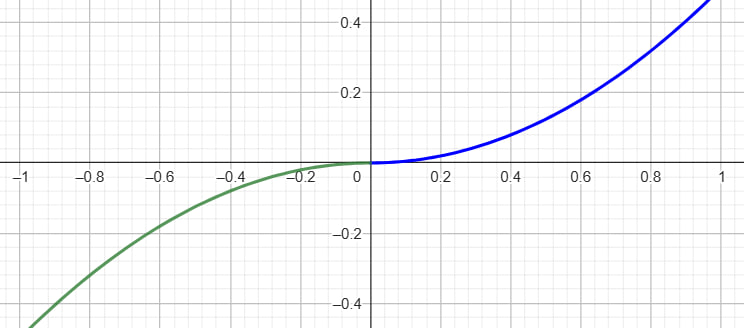
\includegraphics[width=0.7\linewidth]{images/x^2.jpg}
    \caption{График функции $f(x)$, эта функции непрерывна и дифференцируема в точке $x_0=0$, но вторая производная в этой точке у этой функции не существует.}
    \label{fig:enter-label}
\end{figure}

Имеем
\[
 f'(x) = \begin{cases}
     x, & x \ge 0,\\
     -x, & x \le 0
 \end{cases} = |x|,
\]
а как мы уже знаем, (см. Пример \ref{|x|is_not_diff}, эта функция уже не дифференцируема в точке $x=0.$

\begin{figure}
    \centering
    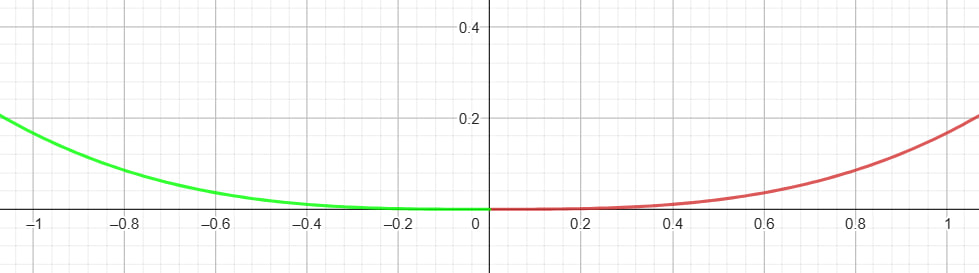
\includegraphics[width=0.7\linewidth]{images/x^3.jpg}
    \caption{Функция $g(x)$ дважды, но трижды дифференцируема в точке $x_0=0$.}
    \label{fig:enter-label}
\end{figure}

Аналогично можно показать, что функция
\[
 g(x) = \begin{cases}
     \dfrac{1}{6} x^3, & x \ge 0,\\
     -\dfrac{1}{6} x^3, & x \le 0,
 \end{cases}
\]
дважды, но не трижды дифференцируема в точке $x_0=0$.
\end{example}


\begin{remark}
    С другой стороны, ясно, что если функция имеет $n$-ую производную, то значит, она имеет $n-1$-ую производную, а значит и $n-2$-ую \textit{и.т.д.}
\end{remark}

Множество всех $n$-раз дифференцируемых функций на множестве $X \subseteq \mathbb{R}$ принято обозначать так $C^n(X)$, при этом, полагают, что $C^0(X)$ -- множество всех непрерывных функций на $C$.

Согласно Теореме \ref{ariph_for_der}, эти множества есть векторные пространства над $\mathbb{R}$, при этом $C^{m}(X)$ -- подпространство в $C^n(X)$, при $m \ge n$. Таким образом, имеем цепочку подпространств 
\[
 C^0(X) \supseteq C^1(X) \supseteq C^2(X) \supseteq \ldots,
\]

\begin{definition}
Если функция дифференцируема сколь угодно много раз на множестве $X\subseteq \mathbb{R}$, то такую функцию называют \textit{гладкой на $X$.} Пространство гладких функций на $X$ обозначают так $C^\infty(X).$ 
\end{definition}

Примерами гладких функций на $\mathbb{R}$ являются любые полиномы, а также функции $\sin(x)$, $\cos(x)$, $\mathrm{exp}(x)$.



\subsection{Полином Тейлора от одной переменной}

Рассмотрим полином $P(x) \in \mathbb{R}[x]$. Говорят, что полином $P(x)$ \textit{разложен в точке $a$ по степеням $(x-a)$}, если существуют такие $c_0, c_1, \ldots, c_n$, где $n = \mathrm{deg}(P(x))$, что $P(x) = c_0 + c_1(x-a) + c_2(x-a)^2 + \cdots + c_n(x-a)^n$. 

Нетрудно видеть, что эти коэффициенты можно найти следующим образом
\[
 c_0 = P(a), \quad c_1 = P'(a), \quad c_2 = \frac{1}{2}P''(a), \quad c_3 = \frac{1}{6}P'''(a), \ldots,  c_n = \frac{1}{n!}P^{(n)}(a).
\]

Таким образом, получаем
\[
 P(x) = P(a) + P'(a)(x-a) + \frac{1}{2} P''(a)(x-a)^2 + \cdots + \frac{1}{n!}P^{(n)}(a)(x-a)^n.
\]


\begin{definition}
    Пусть $f(x)$ есть $n$-раз дифференцируема в точке $a\in \mathbb{R}$. Полином вида 
    \[
     T_f(x): = \sum_{k=0}^n \frac{f^{(k)}(a)}{k!}(x-a)^k
    \]
    называется \textit{полиномом Тейлора для функции $f$}.
\end{definition}


\begin{theorem}
    Если $f$ есть $n$-раз дифференцируемая функция в точке $a$, то
    \[
     f(x) = T_f(x) + o((x-a)^n), \qquad x \to a.
    \]
\end{theorem}

\begin{proof}
    Пусть $r(x): = f(x) - T_f(x)$, очевидно, что $r(a) = r'(a) = \cdots = r^{(n)}(a) = 0$. По правилу Лопиталя \ref{Lop}
    \begin{eqnarray*}
        \lim_{x \to a} \frac{r(x)}{(x-a)^n} &=& \lim_{x \to a} \frac{r'(x)}{n(x-a)^{n-1}} \\
        &=& \lim_{x \to a} \frac{r''(x)}{n(n-1)(x-a)^{n-2}} = \cdots \\
        &=& \lim_{x \to a} \frac{r^{(n-1)}(x)}{n!(x-a)}
    \end{eqnarray*}
Дальше правило Лопиталя применять вообще говорят нельзя, так как по условию известно, что существует лишь $f^{(n)}(a)$, а в окрестности она может не существовать. 

Воспользуемся теперь определением, получаем
\[
 r^{(n)}(a) = \lim_{x \to a} \frac{r^{(n-1)}(x) - r^{(n-1)}(a)}{(x-a)} = \lim_{x \to a} \frac{r^{(n-1)}(x)}{(x-a)},
\]
потому что $r^{(n-1)}(a) = 0$, но тогда
\[
 \lim_{x \to a} \frac{r^{(n-1)}(x)}{n!(x-a)} = \frac{1}{n!}\lim_{x \to a} \frac{r^{(n-1)}(x)}{x-a} = \frac{1}{n!} r^{(n)}(a)= 0,
\]
что и доказывает требуемое.
\end{proof}

\begin{theorem}[Общий вид остаточного монома]\label{gen_monom}
    Пусть $f$ есть $n$ раз дифференцируема в каждой точке отрезка $[a,x]$, функция $f^{(n)}$ непрерывна на $[a,x]$ и дифференцируема на интервале $(a,x)$. Пусть $g(x)$ непрерывна на $[a,x]$ и дифференцируема на $(a,x)$, причём $g\ne 0$ на $(a,x)$. Тогда существует такое $c\in (a,x)$, что
    \[
     f(x) = \sum_{k=0}^n \frac{f^{(k)}(a)}{k!}(x-a)^k + r_n(x,a),
    \]
    где 
    \[
     r_n(x,a) = \frac{1}{n!}\frac{f^{(n+1)}(c)}{g'(c)}\bigl(g(x) - g(a)\bigr)(x-c)^n.
    \]
\end{theorem}
\begin{proof}
Пусть
\begin{eqnarray*}
  \psi(t) &:=& f(x) - \sum_{k=0}^n \frac{f^{(k)}(t)}{k!}(x-t)^k \\
  &=& f(x) - \left(f(t) + f'(t)(x-t) + \cdots + \frac{1}{n!}f^{(n)}(t)(x-t)^n \right) 
\end{eqnarray*}
где $a \le t \le x$.

Тогда
\[
 \psi(x) = 0, \qquad \psi(a) = f(x) - \sum_{k=0}^n \frac{f^{(k)}(a)}{k!}(x-a)^k,
\]
\textit{т.е.,} $r_n(x,a) = \psi(a)$.

Согласно условиям, $\psi(t)$ дифференцируема на $[a,x]$, тогда по теореме Коши \ref{Coushy_for_functions}, существует такое $c \in (a,x)$, что
\[
 \frac{\psi(x)-\psi(a)}{g(x) - g(a)} = \frac{\psi'(c)}{g'(c)},
\]
тогда
\[
 \psi(a) = - \frac{\psi'(c)}{g'(c)}(g(x) - g(c))
\]
поэтому
\[
 r_n(x,a)= - \frac{\psi'(c)}{g'(c)}(g(x) - g(c)).
\]

Имеем
\begin{eqnarray*}
    \psi'(t) &= & - \left( f(t) + f'(t)(x-t) + \frac{1}{2!}f''(t)(x-t)^2 + \frac{1}{3!}f'''(t)(x-t)^3 + \cdots \frac{1}{n!}f^{(n)}(t) (x-t)^n \right)' \\
    &=& -f'(t) \\
    && - f''(t)(x-t) + f'(t) \\
    && - \frac{1}{2!}f'''(t)(x-t)^2 + f''(t)(x-t) \\
    &&  - \frac{1}{3}f^{(4)}(x-t)^3 + \frac{1}{3!}f'''(t)(x-t)^3 \\
    && \cdots - \frac{f^{(n+1)}(t)}{n!}(x-t)^n \\
    &=& - \frac{f^{(n+1)}(t)}{n!}(x-t)^n.
\end{eqnarray*}

Таким образом,
\[
 r_n(x,a) =\frac{1}{n!}\frac{f^{(n+1)}(c)}{g'(c)}\bigl(g(x) - g(a)\bigr)(x-c)^n,
\]
что и требовалось доказать.    
\end{proof}


\begin{corollary}[Остаточный моном в форме Коши]
    \[
     \begin{boxed}{
         r_n(x,a) = \frac{f^{(n+1)}(c)}{n!}(x-a)(x-c)^n, \quad a < c <x.}
     \end{boxed}
    \]
\end{corollary}
\begin{proof}
    Нужно положить $g(x) = x-t$ в теореме \ref{gen_monom}.
\end{proof}

\begin{corollary}[Остаточный моном в форме Лагранжа.]\label{monom_in_Langrange}
    \[
     \boxed{
      r_n(x,a) = \frac{f^{(n+1)}(c)}{(n+1)!}(x-a)^{n+1}, \qquad a < c <x.
     }
    \]
\end{corollary}
\begin{proof}
    Нужно положить $g(x) = (x-t)^{n+1}.$
\end{proof}


\subsection{Выпуклость и вогнутость}

\begin{definition}
 Функция $f:[a,b] \to \mathbb{R}$, называется \textit{выпуклой на отрезке} $[a,b]$, если для любых $x_1,x_2 \in [a,b]$ выполняется неравенство
 \[
  f \left( \frac{x_1+x_2}{2} \right) \le \frac{f(x_1) + f(x_2)}{2}.
 \]

 Функция $f(x)$ называется \textit{вогнутой на отрезке} $[a,b]$, если функция $-f(x)$ ---выпукла на $[a,b].$
\end{definition}

\begin{lemma}\label{convex_for_n}
 Если $f:[a,b] \to \mathbb{R}$ -- выпукла, то для любых $x_1,\ldots, x_n \in [a,b]$,
 \[
  f \left( \frac{x_1+ \cdots + x_n}{n} \right) \le \frac{f(x_1) + \cdots + f(x_n)}{n}.
 \]
\end{lemma}
\begin{proof}
 Это сразу следует из определения выпуклости и применения метода индукции. 
\end{proof}

\begin{proposition}\label{convex_proposition}
    Пусть $f:[a,b] \to \mathbb{R}$ -- выпукла на $[a,b]$, $p,q \ge 0$, $p+q=1$.
    \begin{enumerate}
        \item Если $p,q\in \mathbb{Q}$, то $f(px_1 + qx_2) \le p f(x_1) + q f(x_2)$.
        \item Если $f$ -- непрерывна на $[a,b]$, то 
        \[
         f(px_1 + qx_2) \le p f(x_1) + q f(x_2),
        \]
 для любых $p,q \ge 0$, с условием $p+q=1$.
    \end{enumerate}
\end{proposition}

\begin{proof}~

(1)  Пусть $p,q \in \mathbb{Q}$, тогда, в виду условия $p+q=1$, имеются такие $m \in \mathbb{Z}_+$, $n \in \mathbb{N}$, что $p = \frac{m}{n}$, $q = \frac{n-m}{n}$.

По лемме \ref{convex_for_n}, получаем
\begin{eqnarray*}
 f(px_1 + qx_2) &=& f\left( \frac{m}{n}x_1 + \frac{n-m}{n} x_2 \right) = f\left( \frac{mx_1 + (n-m)x_2}{n} \right) \\
 &=&   f\Bigl( \frac{\overbrace{x_1 + \cdots +x_1}^m + \overbrace{x_2 + \cdots +x_2}^{n-m}}{n}\Bigr)  \\
 &\le& \frac{mf(x_1) + (n-m)f(x_2)}{n} \\
 &=& \frac{m}{n} f(x_1) + \frac{n-m}{n} f(x_2) \\
 &=& pf(x_1) + q f(x_2),
\end{eqnarray*}
что и требовалось доказать.

(2) Пусть теперь $f$ -- непрерывна на отрезке $[a,b]$, и пусть $p,q \in \mathbb{R}$, $p,q \ge 0$, $p+q =1$. Так как $\overline{\mathbb{Q}} = \mathbb{R}$ (см. отдел \ref{barQ=R}), то можно найти такие последовательности $(p_n)$, $(q_n)$ положительных рациональных чисел $p_n, q_n \in \mathbb{Q}$, что $\lim_{n\to \infty} p_n = p$, $\lim_{n\to \infty}q_n =q$.\footnote{Можно и проще, так как моделью $\mathbb
R$ являются бесконечные десятичные дроби, то если, скажем, 
$$p = \alpha_0. \alpha_1\alpha_2\alpha_3\cdots$$
бесконечная дробь, то последовательность рациональных чисел 
\[
 \alpha_0, \quad \alpha_0.\alpha_1, \quad  \alpha_0.\alpha_1\alpha_2, \quad \alpha_0.\alpha_1\alpha_2\alpha_3, \quad \ldots
\]
сходится к $p.$
} Более того, согласно теореме \ref{a+b,ca,ab}, $p_n + q_n = 1$ для всех $n \in \mathbb{N}.$

Тогда, согласно Теореме \ref{a+b,ca,ab}, $\lim_{n\to \infty} (p_n x_1 + q_n x_2 ) = pz_1 + q x_2$, и теперь, используя Теорему \ref{lim=>for_any_sequence} (=определение по Гейне), получаем
\begin{equation}\label{convex_theorem_1}
  \lim_{n\to \infty} f(p_n x_1 + q_n x_2) = f(px_1 + qx_2).    
\end{equation}

С другой стороны, согласно теореме \ref{a+b,ca,ab}, получаем
\begin{equation}\label{convex_theorem_2}
  \lim_{n\to \infty} \left( p_n f(x_1) + b_n f(x_2)\right) = p f(x_1) + q f(x_2).    
\end{equation}


Далее, так как $f$ -- выпукла на $[a,b]$, то, согласно доказанному пункту (1), для рациональных чисел $p_n,q_n$, для которых верно $p_n, q_n \ge 0$, $p_n + q_n =1$, имеем
\[
 f(p_nx_1 + q_n x_2) \le p_n f(x_1) + q_n f(x_2),
\]
тогда согласно теореме \ref{lim(f+g)},
\[
\lim_{n\to \infty} f(p_nx_1 + q_n x_2) \le \lim_{n\to \infty} \left( p_n f(x_1) + q_n f(x_2) \right),
\]
учитывая теперь (\ref{convex_theorem_1}), (\ref{convex_theorem_2}), получаем
\[
 f(px_1 + q x_2) \le p f(x_1) + q f(x_2).
\]

Это завершает доказательство.
\end{proof}

\begin{corollary}\label{cor_for_convex}
    Если $f:[a,b] \to \mathbb{R}$ -- непрерывная и выпукла, то для любого $x \in (a,b)$,
    \[
     \frac{f(x) - f(a)}{x-a} \le \frac{f(b) - f(x)}{b-x}.
    \]
\end{corollary}
\begin{proof}
Пусть $p:= \frac{b-x}{b-a}$ и $q: = \frac{x-a}{b-a}$. Видно, что $p,q \ge 0$, и $p+q=1$, тогда согласно предложению \ref{convex_proposition}, для любых $p,q \ge 0$, $p+q=1$, $f(px_1 + qx_2) \le pf(x_1) + qf(x_2)$.

Так как $x = \frac{b-x}{b-a} \cdot a + \frac{x-a}{b-a}\cdot b$, то получаем
\[
 f(x) = f\left(  \frac{b-x}{b-a} \cdot a + \frac{x-a}{b-a}\cdot b\right) \le \frac{b-x}{b-a} f(a) + \frac{x-a}{b-a}f(b).
\]

Таким образом, получаем

\[
 (b-a)f(x) \le (b-x) f(a) + (x-a) f(b).
\]

Далее, так как $b-a = (b-x) - (a-x)$, то можно записать
\[
 (b-a) f(x) = \left( (b-x) - (a-x) \right) f(x) = (b-x)f(x) - (a-x)f(x),
\]
тогда используя неравенство выше, получаем
\[
 (b-x)f(x) - (a-x)f(x) \le (b-x) f(a) + (x-a) f(b),
\]
а это можно переписать так
\[
 (b-x) (f(x) - f(a)) \le (x-a) (f(b) - f(x)),
\]
или что равносильно неравенству 
 \[
     \frac{f(x) - f(a)}{x-a} \le \frac{f(b) - f(x)}{b-x},
    \]
что и требовалось доказать.
\end{proof}

\begin{theorem}
    Пусть $f: [a,b] \to \mathbb{R}$ -- дифференцируемая функция на отрезке $[a,b]$. Тогда $f$ -- выпукла тогда и только тогда, когда $f'$ не убывает на $[a,b]$.
\end{theorem}
\begin{proof}~

(1) Пусть $f$ -- выпукла,  и пусть $a \le x_1 < x < x_2 \le b$, тогда согласно следствию \ref{cor_for_convex}, 
\[
 \frac{f(x) - f(x_1)}{x-x_1} \le \frac{f(x_2) -  f(x)}{x_2- x}.
\]

Тогда, согласно теореме \ref{lim(f+g)} (=предел от неравенств) и определению производной (см. Определение \ref{derivative_of_function}), имеем
\[
 \lim_{x \to x_1} \frac{f(x) - f(x_1)}{x-x_1} =:f'(x_1) \le \lim_{x \to x_1} \frac{f(x_2) -  f(x)}{x_2- x} = \frac{f(x_2) -  f(x_1)}{x_2- x_1}
\]
а также 
\[
 \lim_{x \to x_2}  \frac{f(x) - f(x_1)}{x-x_1} =  \frac{f(x_2) - f(x_1)}{x_2-x_1} \le \lim_{x\to x_2} \frac{f(x_2) -  f(x)}{x_2- x} =: f'(x_2).
\]

Итак, мы получили, что 
\[
 f'(x_1) \le \frac{f(x_2) -  f(x_1)}{x_2- x_1} \le f'(x_2), 
\]
\textit{т.е.,} имеем $f'(x_1) \le f'(x_2)$ для любых $a \le x_1  < x_2 \le b$, а это и доказывает не убывание функции $f'.$

(2) Пусть теперь функция $f'$ не убывает на $[a,b]$, тогда согласно теореме Лагранжа (см. Теорема \ref{Langrange}), для любых $a \le x_1 < x < x_2 \le b$ существуют такие $\theta_1 \in (x_1, x)$, $\theta_2 \in (x,x_2)$, что
\[
 f'(\theta_1) = \frac{f(x) - f(x_1)}{x-x_1}, \qquad f'(\theta_2) = \frac{f(x_2) - f(x)}{x_2-x}.
\]

Так как мы предположили, что $f'$ не убывает на отрезке $[a,b]$ и так как $\theta_1 < \theta_2$, то $f'(\theta_1) \le f'(\theta_2)$, но тогда
\[
 \frac{f(x) - f(x_1)}{x-x_1} \le \frac{f(x_2) - f(x)}{x_2-x},
\]
но согласно следствию \ref{cor_for_convex} это и означает выпуклость функции $f$ на отрезке $[a,b].$ Это завершает доказательство.
\end{proof}

\begin{corollary}
    Если функция $f:[a,b] \to \mathbb{R}$ дважды дифференцируема на $[a,b]$, то $f$ выпукла на $[a,b]$ тогда и только тогда, когда $f''(x) \ge 0$ для любого $x \in [a,b].$
\end{corollary}
\begin{proof}
    Это сразу следует из предыдущей теоремы и критерием возрастания (см. Следствие \ref{monoton_criteria}).
\end{proof}

\begin{definition}
    Точка $x_0 \in [a,b]$ в которой $f''(x_0) =0$ называют \textit{точкой перегиба.}
\end{definition}